\section{Sp\-Glut\-Window.cpp File Reference}
\label{SpGlutWindow_8cpp}\index{SpGlutWindow.cpp@{SpGlutWindow.cpp}}
{\tt \#include \char`\"{}Sp\-Window.h\char`\"{}}\par
{\tt \#include \char`\"{}Sp\-Gl\-Headers.h\char`\"{}}\par
{\tt \#include \char`\"{}Sp\-Glut\-Key\-Bindings.h\char`\"{}}\par
{\tt \#include \char`\"{}Sp\-Glut\-Headers.h\char`\"{}}\par


Include dependency graph for Sp\-Glut\-Window.cpp:\begin{figure}[H]
\begin{center}
\leavevmode
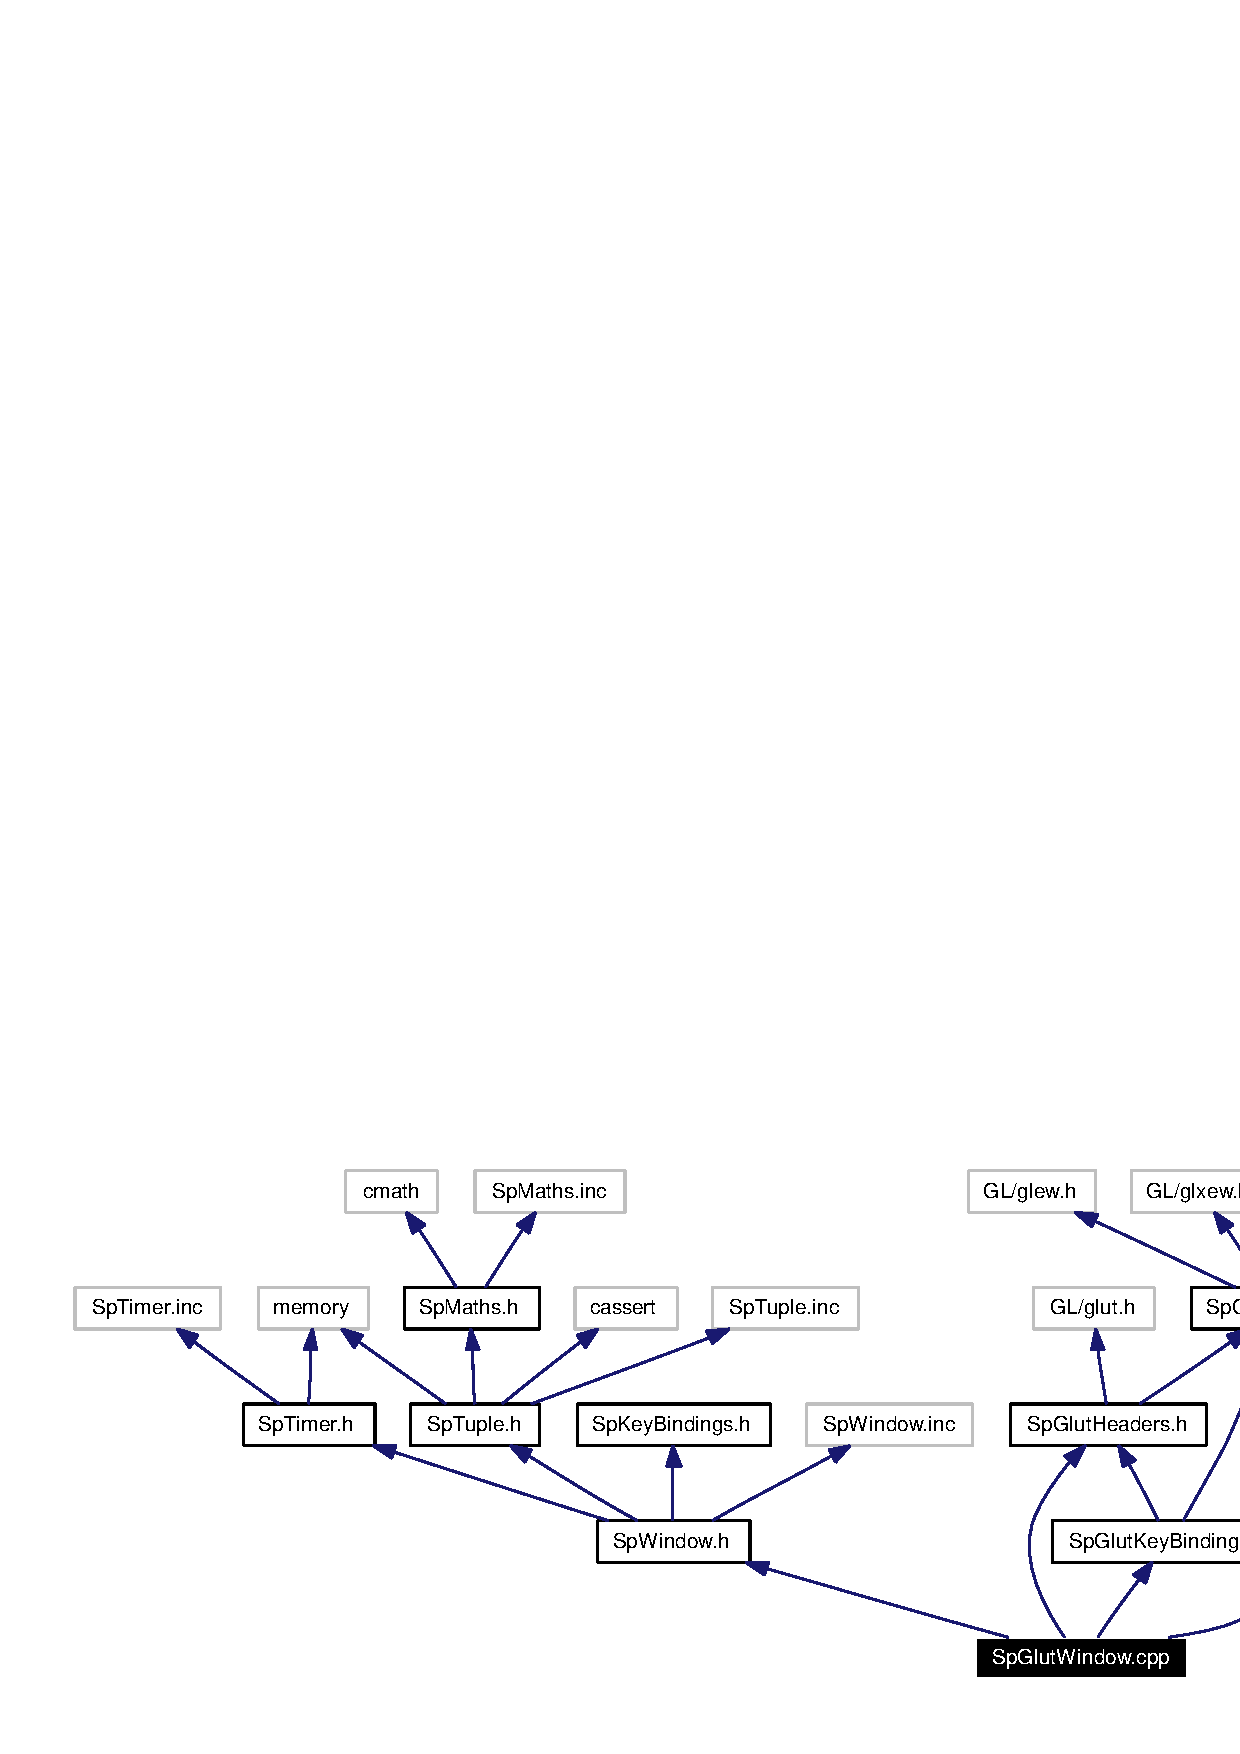
\includegraphics[width=374pt]{SpGlutWindow_8cpp__incl}
\end{center}
\end{figure}
\subsection*{Functions}
\begin{CompactItemize}
\item 
int {\bf main} (int argc, char $\ast$$\ast$argv)
\end{CompactItemize}


\subsection{Function Documentation}
\index{SpGlutWindow.cpp@{Sp\-Glut\-Window.cpp}!main@{main}}
\index{main@{main}!SpGlutWindow.cpp@{Sp\-Glut\-Window.cpp}}
\subsubsection{\setlength{\rightskip}{0pt plus 5cm}int main (int {\em argc}, char $\ast$$\ast$ {\em argv})}\label{SpGlutWindow_8cpp_a13}


Definition at line 272 of file Sp\-Glut\-Window.cpp.

References Spark::Sp\-Window::current(), Spark::Sp\-Window::height(), Spark::Sp\-Window::id(), Spark::Sp\-Window::on\-Initialize(), Spark::Sp\-Window::on\-Startup(), Spark::Sp\-Window::set\-Window\-Id(), Spark::Sp\-Window::title(), and Spark::Sp\-Window::width().